\documentclass{jsarticle}
\usepackage[dvipdfmx]{graphicx}
\usepackage{subcaption}
\captionsetup[figure]{justification=centering}
\captionsetup[table]{justification=centering}
\usepackage[ipa]{pxchfon}
\usepackage{float}
\usepackage[margin=20truemm]{geometry}


\begin{document}
\title{{\vspace*{-10mm}}{\LARGE 0629課題}}
\author{\large 千葉工業大学 先進工学部 未来ロボティクス学科 \vspace*{4mm}\\20C1015 今井悠月}
\date{}
\maketitle\vspace*{10mm}
\vspace*{-10mm}

\section*{問}
本日学んだカルマンフィルタを用いた自己位置推定を応用して, octaveを使用して自己位置推定の様子を確認せよ.

\section*{解答}

\begin{figure}[H]
  \centering
   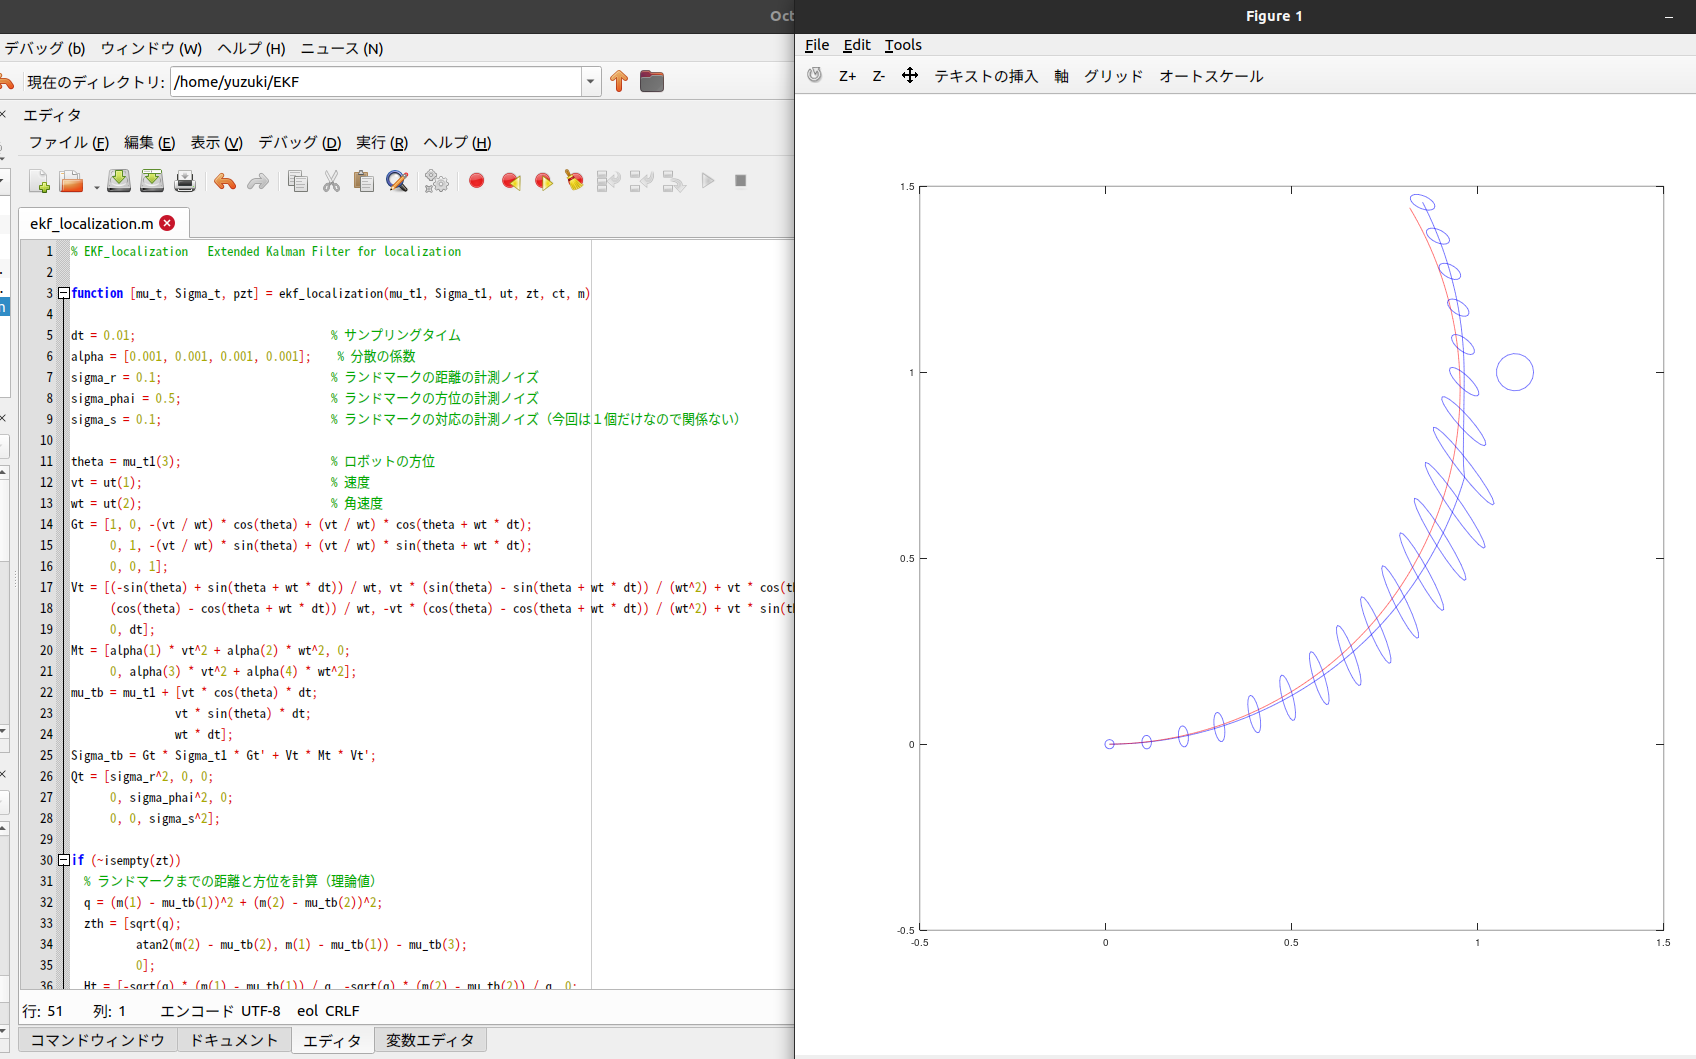
\includegraphics[scale=0.30]{./fig/1.png}
   \caption{実行結果のグラフ}
\end{figure}

\begin{figure}[H]
  \centering
   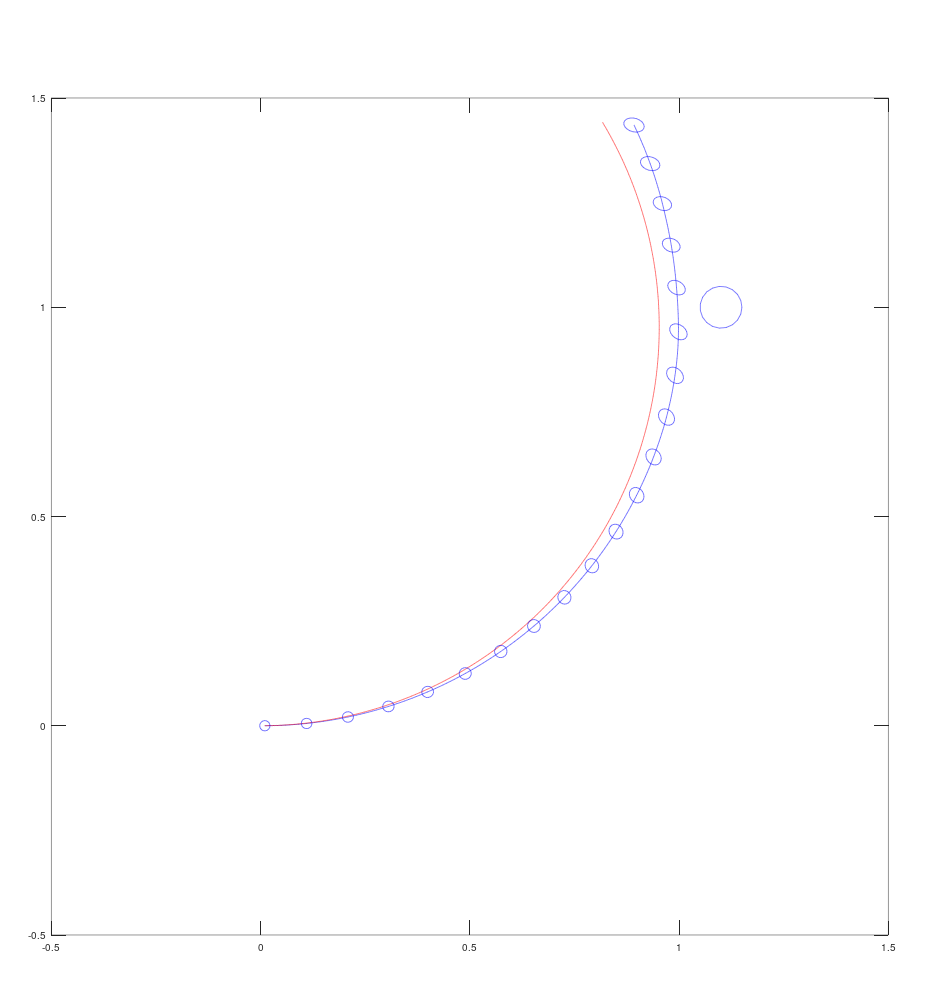
\includegraphics[scale=0.5]{./fig/2.png}
   \caption{条件を変えて計算した時のグラフ}
\end{figure}

\subsection*{変更した条件と簡単なコメント}
ekf\_localization\_main.m 中の Sigma\_t(共分散行列)の対角成分をすべて\( 0.005^2 \)に変更\\
\hspace*{1zw}誤差楕円は全体的に小さくなったが, 誤差楕円内に真値が含まれていない箇所が多くなった.
\end{document}